\newprob{1715421793}
{
    % Physics At Work(Physics In Life 2ed) Question Bank/2_ch05_LQ_e Q1
    一個邊長為 0.3 m 的正方形板塊$ABCD$被釘在牆上的$B$點懸掛,如圖所示。該板塊可以自由地圍繞$B$點旋轉。三個外力分別作用在三個角落$A$、$B$和$C$上,以保持板塊處於平衡狀態。 \bigskip
    \par{\par\centering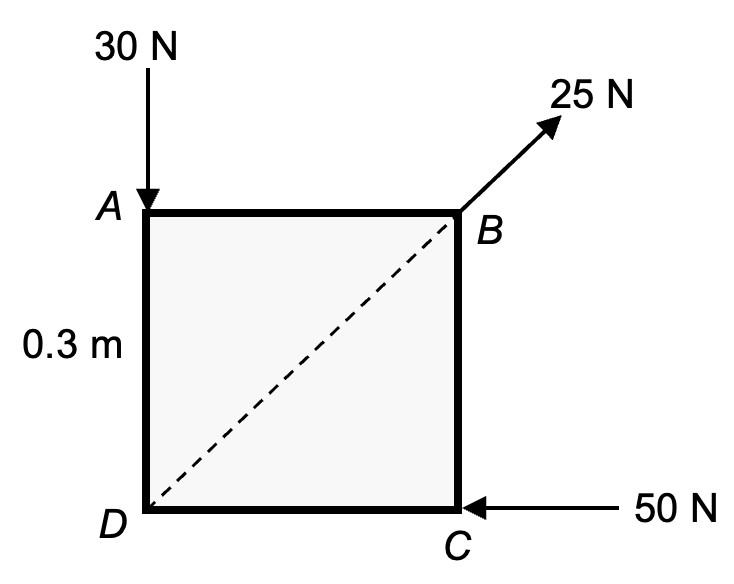
\includegraphics[width=.4\textwidth]{./img/ch3_moment_lq_2024-05-11-20-17-12.png}\par} \bigskip
    \begin{parts}
        \part 在圖中標示板塊的重心位置 $O$。\zzh{1}
        \part 若移除其中一個外力,該板塊仍然可以保持平衡。這是哪一個外力呢?解釋你的答案。 \zzh{2}
        \part 求板塊的質量。\zzh{2}
        \part 如果(b)中提到的外力被移除,請找出釘子對木板施加的力的量值和方向。\zzh{4}
        \part 如果所有三個外力都被移除,請畫圖來顯示木板是如何被釘子懸掛的。\zzh{1}
    \end{parts}
    % \dlines{1}\clearpage \dlines{1}
}{
    % \begin{tabularx}{\linewidth}{|X|l|l|}
    %     \hline
    %     \textbf{答案}                                        &
    %     \textbf{分數}                                        &
    %     \textbf{說明} \\ \hline \hline
    %     \begin{msenum}
    %         \item \topalignc{\par\centering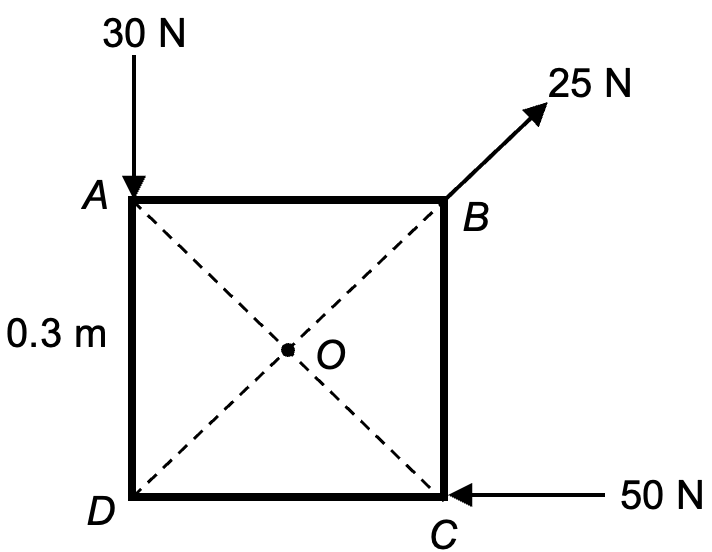
\includegraphics[width=.3\textwidth]{./img/ch3_moment_lq_2024-05-11-19-04-48.png}\par}
    %     \end{msenum} &

    %                     \\
    %     $\displaystyle{=\frac{3x^2-3x+2x-2}{(x-1)(x+1)}}$} & B1      \\ \hline
    %     2                                                  & Row 2 & \\ \hline
    %     3                                                  & Row 3 & \\ \hline
    %     4                                                  &       & \\ \hline
    % \end{tabularx}
    % \par{\par\centering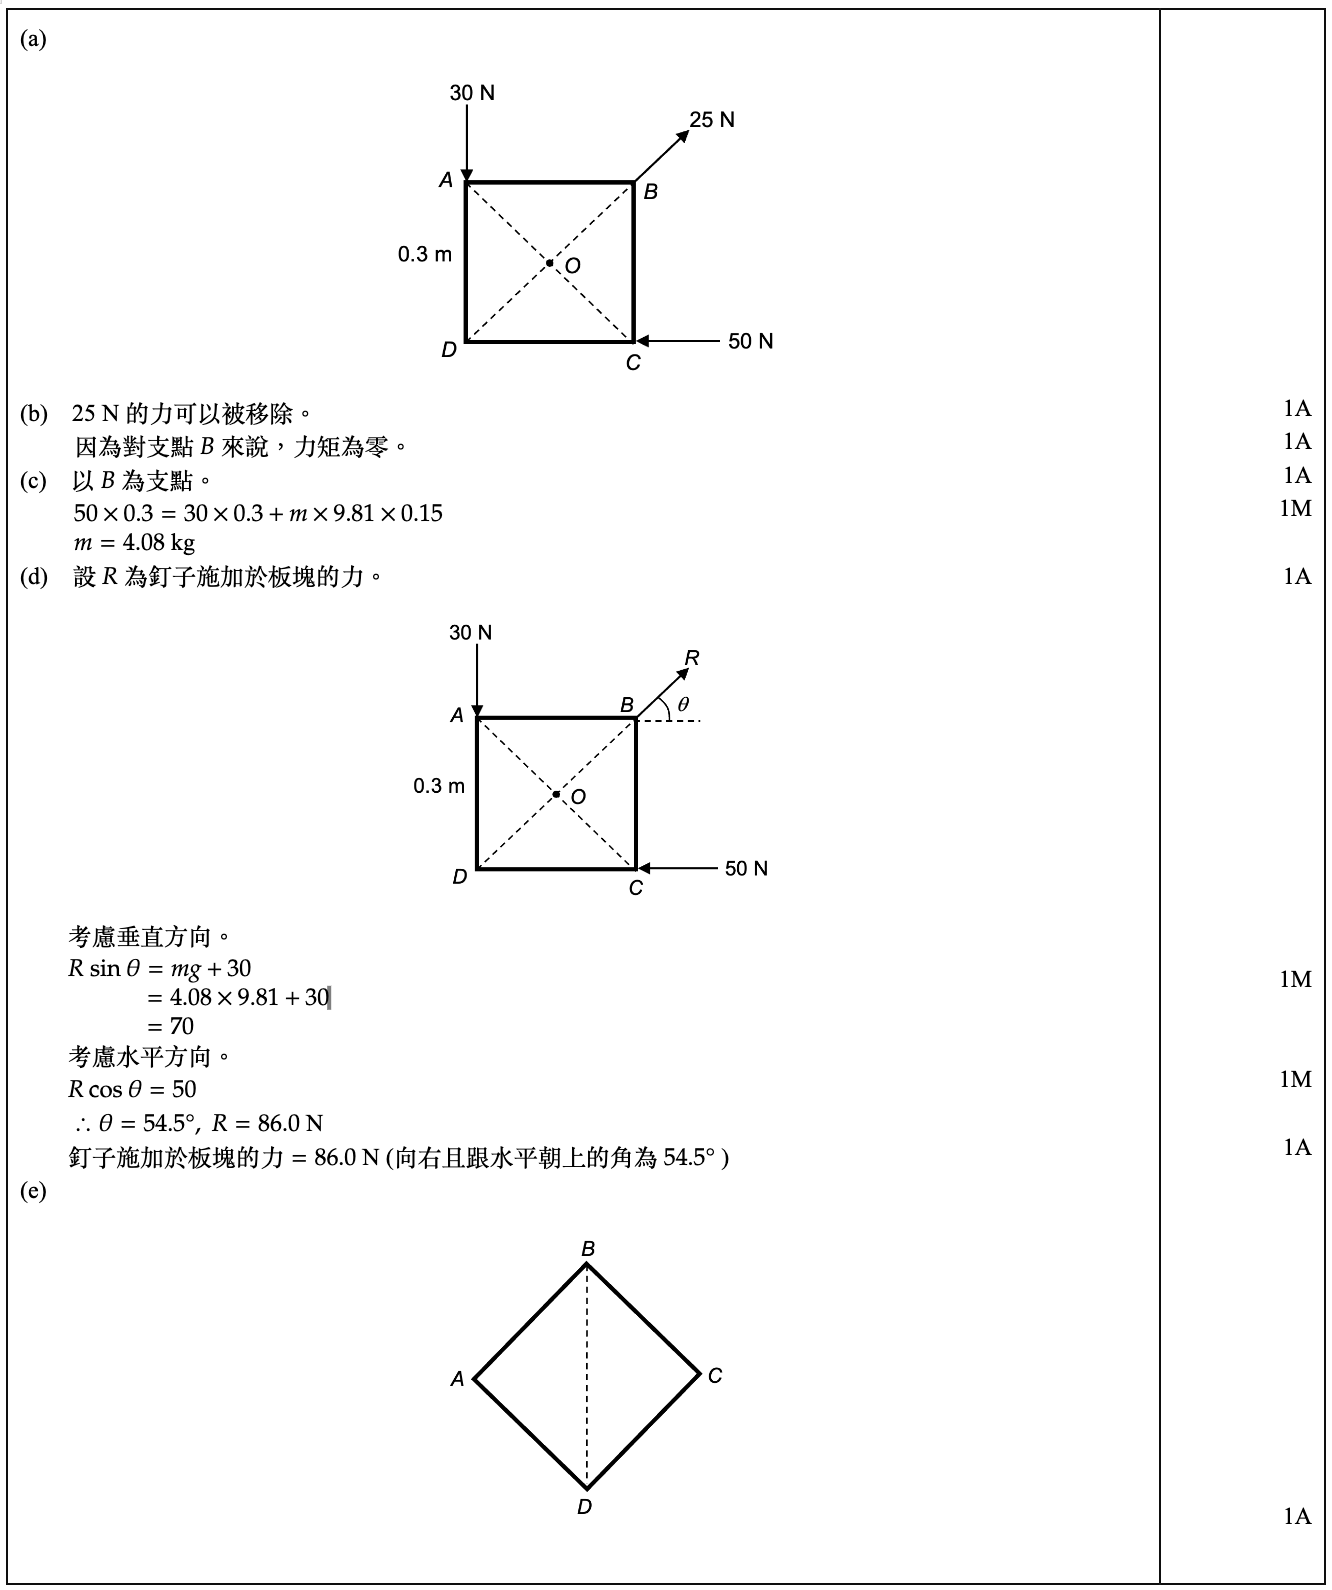
\includegraphics[width=\textwidth]{./img/ch3_moment_lq_2024-05-11-19-28-29.png}\par}
    \sol\par{\par\centering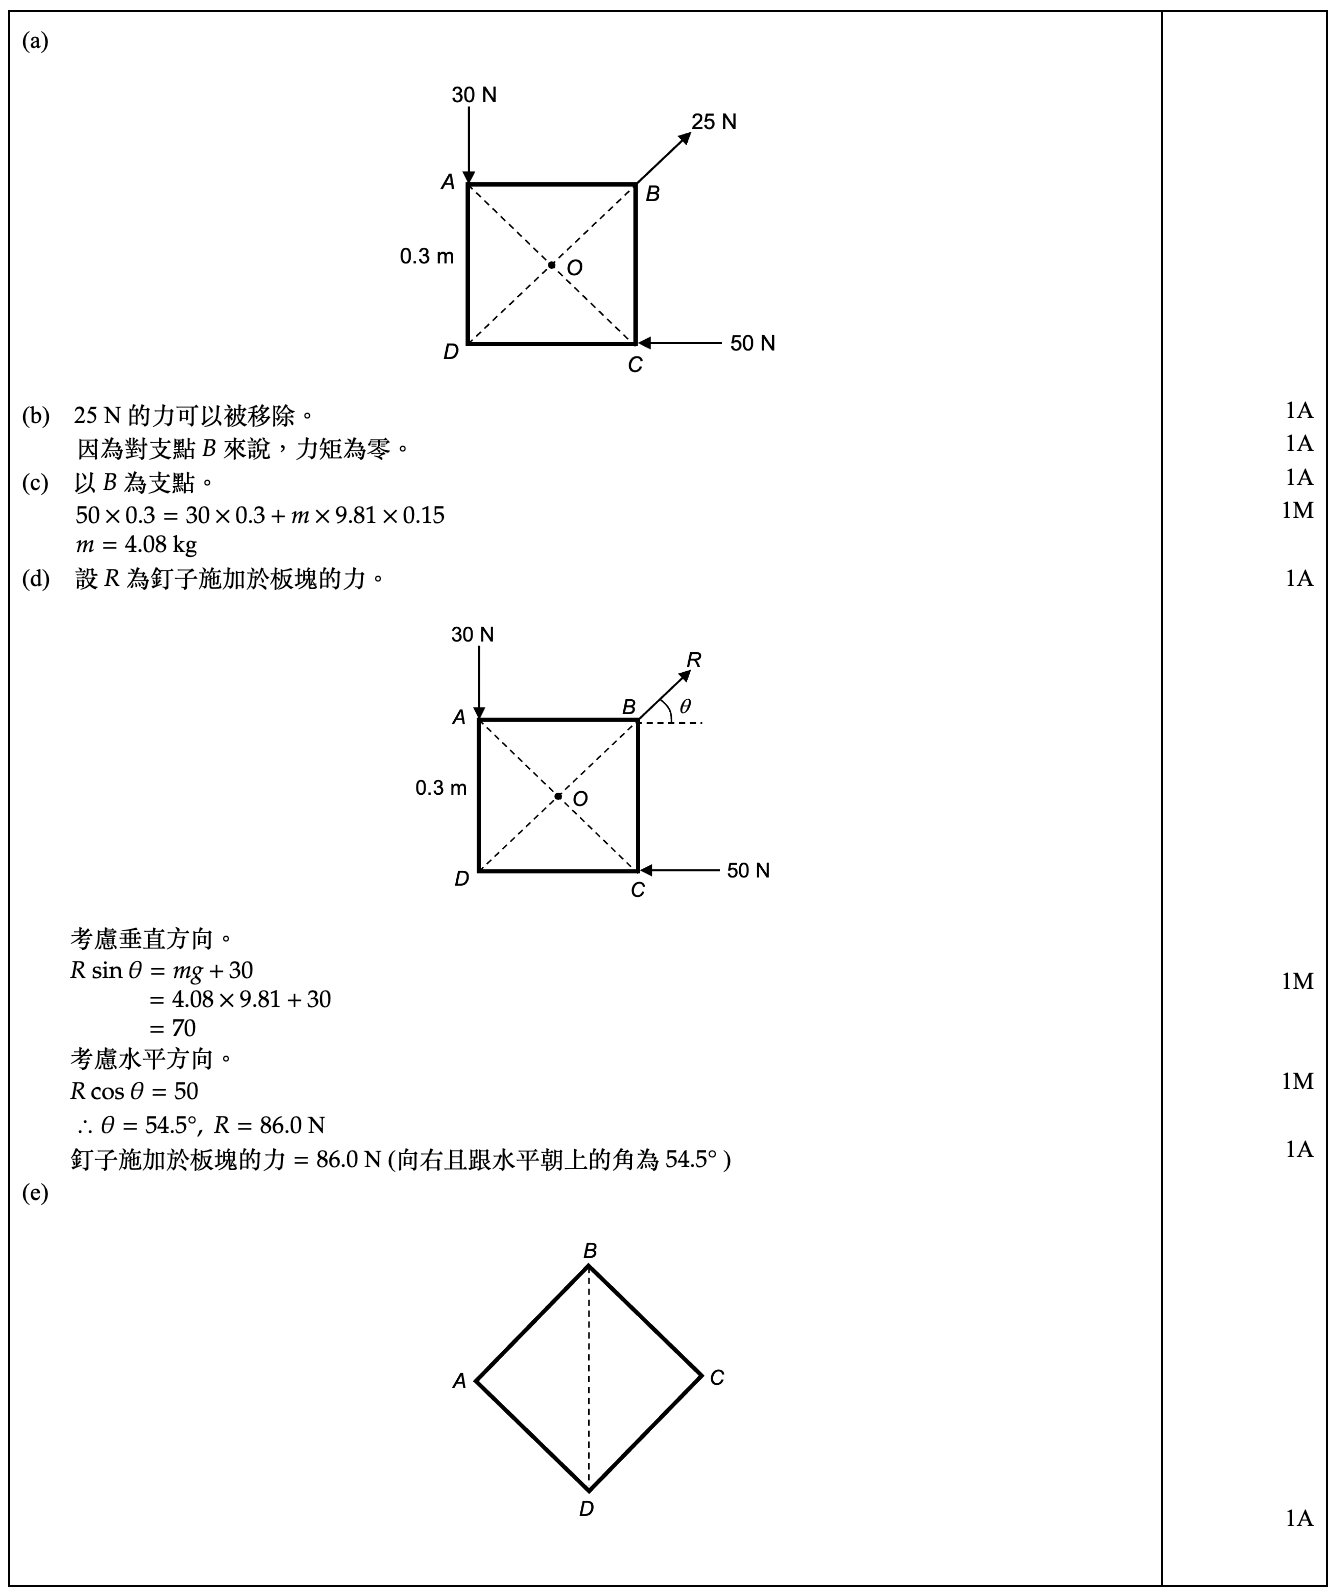
\includegraphics[width=\textwidth]{./img/ch3_moment_lq_2024-05-11-19-29-19.png}\par}
}

% \newprob{1715427313}
% {
%     % Jimmy’s dad drives him home. At a turning, his dad turns the steering wheel clockwise with both hands. The force applied by each hand is 10 N and they form a couple. The diameter of the steering wheel is 30 cm.
%     吉米的爸爸載他回家。在一個轉彎處,他的爸爸用雙手順時針轉動方向盤。每隻手施加的力為 10 N,它們形成一對力偶。方向盤的直徑為 30 cm。\bigskip
% \par{\par\centering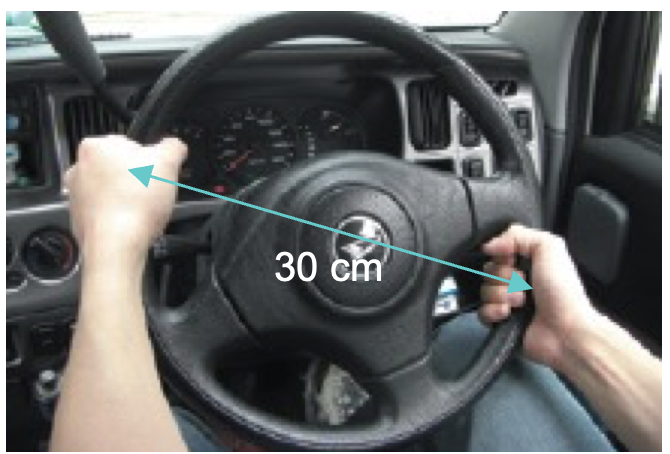
\includegraphics[width=.3\textwidth]{./img/ch3_moment_lq_2024-05-11-19-38-20.png}\par}\bigskip
% \begin{parts}
%     \part 在以下的圖中,繪畫把吉米的爸爸對方向盤施加的力在出來。
% \end{parts}
% }{}

\newprob{1715428454}
{
    %active physics p198 22
    一塊長板重量為100 N,長度為3 m,傾斜地擱在 一道平滑垂直牆壁的$A$點上,另一端則放在粗糙 地面的 $B$點上。
    \bigskip\par{\par\centering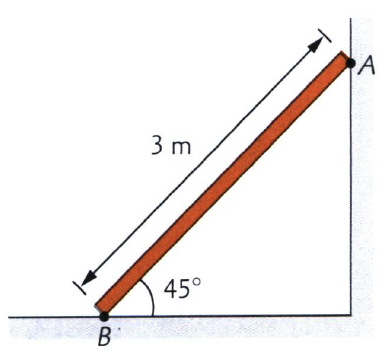
\includegraphics[width=.3\textwidth]{./img/ch3_moment_lq_2024-05-11-19-54-31.png}\par}\bigskip
    \begin{parts}
        \part 求地面作用在長板上的法向反作用力。\zzh{1}
        \part 牆壁作用在長板上的法向反作用力是多少?\zzh{2}
        \part 求長板與地面之間的摩擦力。\zzh{1}
        \part 現在,把長板擱在牆壁的$A'$點上,另一端則 滑到地面的$B'$上。$\theta<45^\circ$。
        \par{\par\centering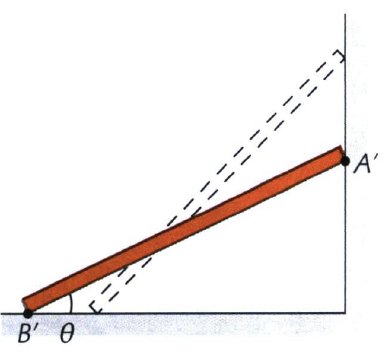
\includegraphics[width=.3\textwidth]{./img/ch3_moment_lq_2024-05-11-19-56-40.png}\par}
        (b)部及(c)部的答案會有何改變?試扼要解 釋。 \zzh{2}
    \end{parts}
    % \dlines{1}\clearpage\dlines{1}
}{
    \sol
    \par{\par\centering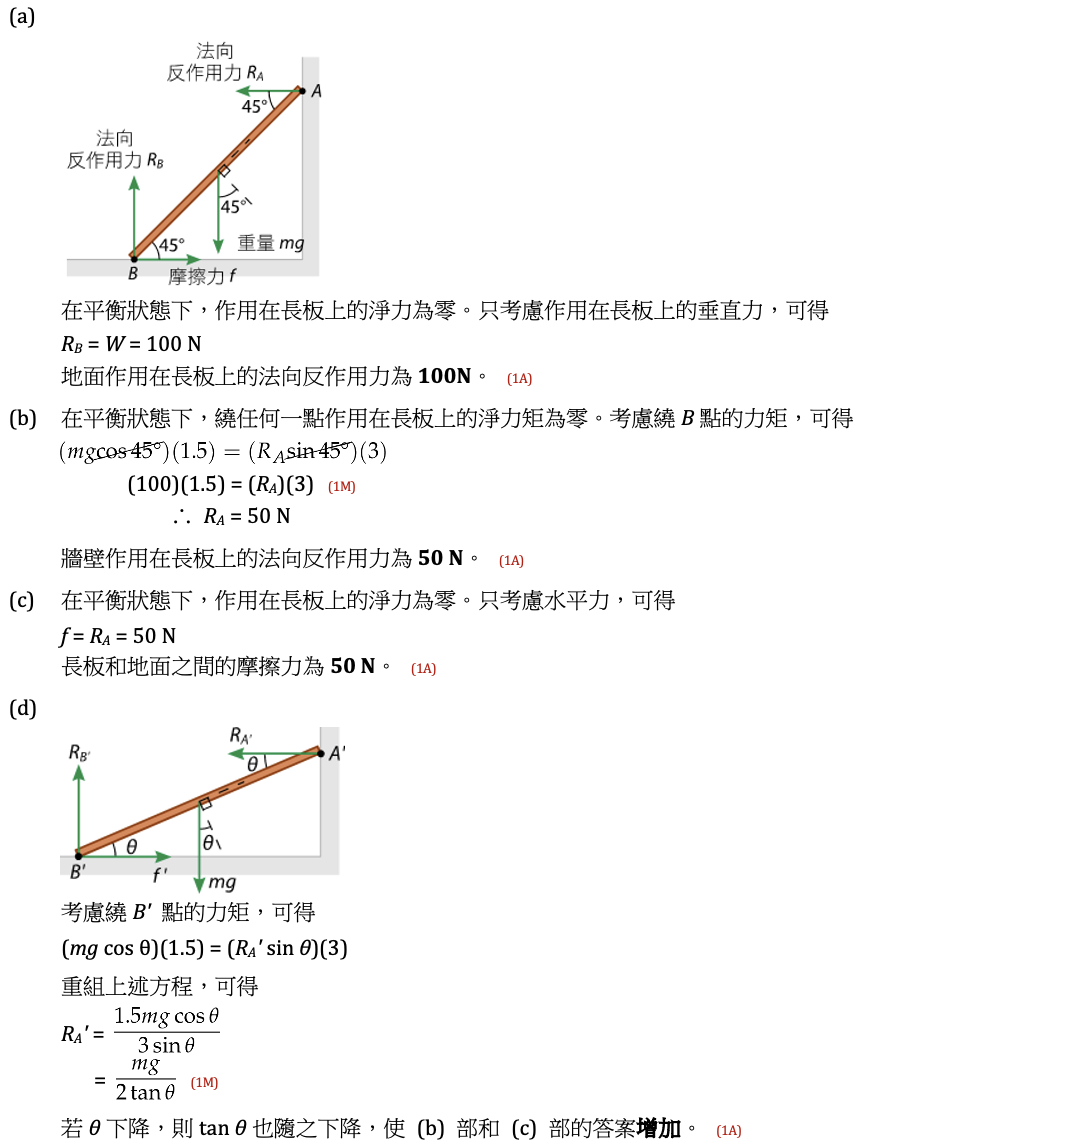
\includegraphics[width=\textwidth]{./img/ch3_moment_lq_2024-05-11-20-25-11.png}\par}
}

\newprob{1715428745}
{
    %active physics p198 23
    圖(a)顯示,偉業正彎身提起一個重物$L$ (= 100 N), 脊椎與垂直方向之間的夾角為 \dg{60}。
    % \par{\par\centering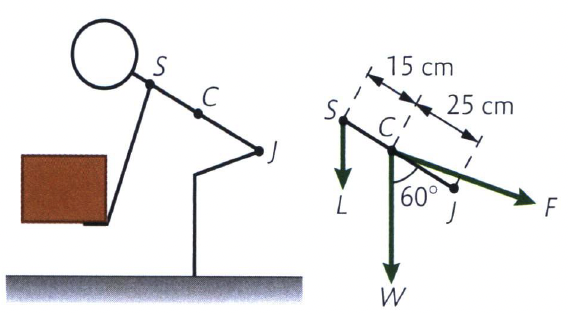
\includegraphics[width=\textwidth]{./img/ch3_moment_lq_2024-05-11-20-00-06.png}\par}
    % \begin{figure}[h!]
    %     \centering
    %     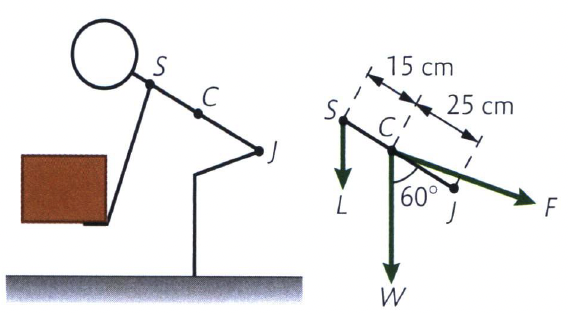
\includegraphics[width=.45\textwidth]{./img/ch3_moment_lq_2024-05-11-20-00-06.png}
    %     \caption{}
    % \end{figure}
    \par{\par\centering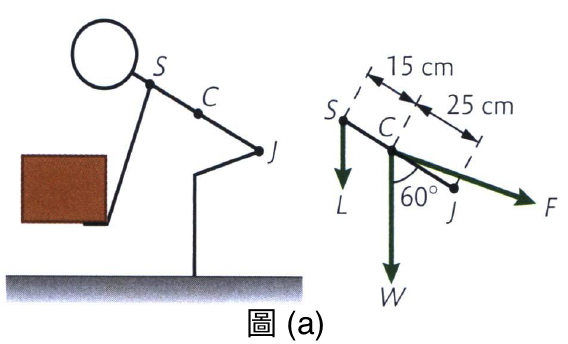
\includegraphics[width=.4\textwidth]{./img/ch3_moment_lq_2024-05-11-20-03-15.png}\par}
    偉業上半身的重量$W$ ( = 400 N) 作用在$C$點上, 與關節$J$相距 25 cm。背部的肌肉提供的合力$F$ 作用在$C$點上,並與脊椎成固定的 \dg{10} 夾角。假 設重物的重量垂直作用在$S$點,而$S$、$C$兩點相 距 15 cm。
    \begin{parts}
        \part 考慮繞關節$J$的力矩,若要偉業維持如此姿 勢,力$F$需為多少? \zzh{2}
        \part 現在,偉業屈膝蹲下以提起相同的重物,如 圖(b)所示。假如脊椎與垂直方向之間的夾角 現為 \dg{30},新的力$F$為多少? \zzh{2}
        \par{\par\centering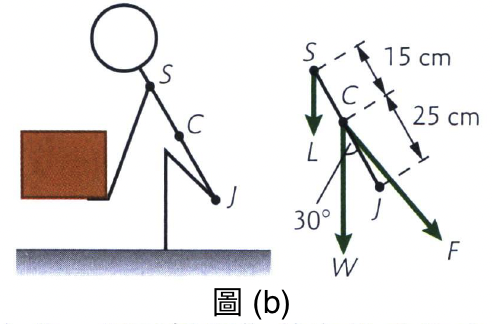
\includegraphics[width=.4\textwidth]{./img/ch3_moment_lq_2024-05-11-20-06-05.png}\par}
        \part 由此,扼要解釋為甚麼搬重物時,應盡量使 重物與雙足靠近。\zzh{2}
    \end{parts}
    % \dlines{1}\clearpage\dlines{1}
}{
    \sol{\par\centering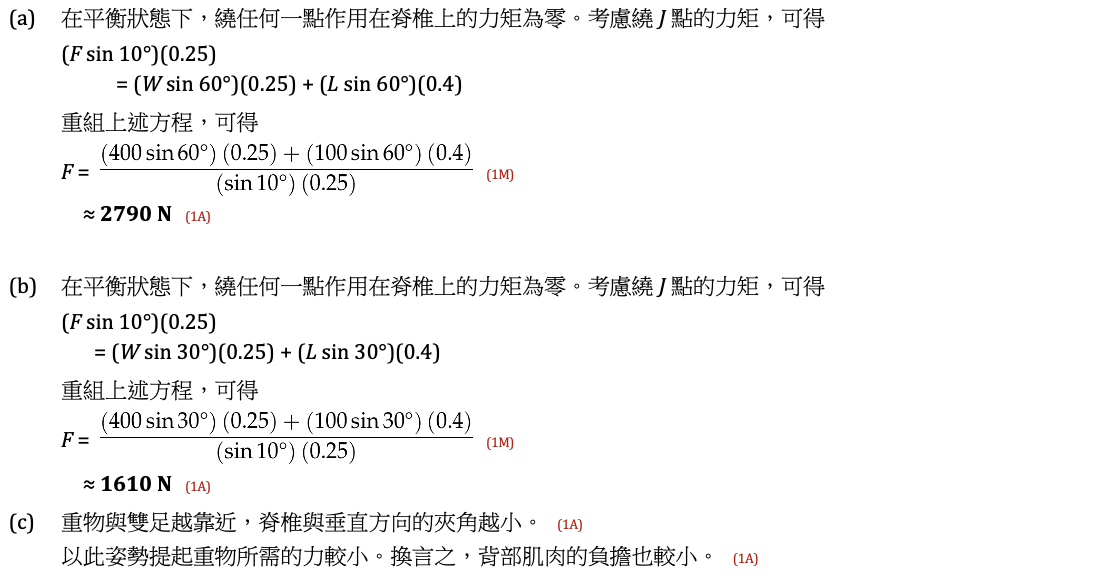
\includegraphics[width=\textwidth]{./img/ch3_moment_lq_2024-05-11-20-24-08.png}\par}
}

\newprob{1715429328}
{
    %active physics p201 * 3
    兩塊完全相同的方塊$X$和$Y$長度同為24 cm,如下圖般在一個桌面上疊起。方塊$X$ 伸出方塊$Y$的 長度為$a_1$,而方塊Y伸出桌面的長度則為$a_2$。忽 略方塊之間的摩擦力。
    \par{\par\centering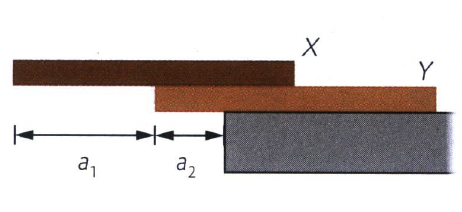
\includegraphics[width=.35\textwidth]{./img/ch3_moment_lq_2024-05-11-20-12-17.png}\par}
    \begin{parts}
        \part 在下列情況中,指出有關重心的情況。
        \begin{subparts}
            \subpart 方塊$X$不會從方塊$Y$上翻倒時,方塊$Y$ 的重心 \zzh{1}
            \subpart 兩個方塊不會從桌面翻倒時,方塊系統 的重心 \zzh{1}
        \end{subparts}
        \part 調整兩個方塊的位置,使方塊$X$伸出至最遠 而不翻倒。求此情況下的長度$a_1$和 $a_2$ 。\zzh{3}
        \part 把第三個方塊$Z$插入方塊$Y$下,如下圖所 示。在方塊$X$伸出至最遠而不翻倒的情況 下,求$a_3$。 \par\zzh{1}
        \par{\par\centering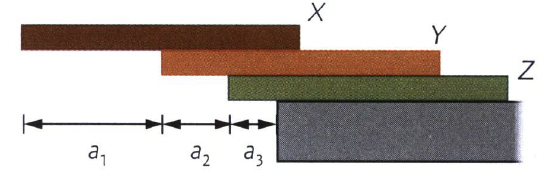
\includegraphics[width=.4\textwidth]{./img/ch3_moment_lq_2024-05-11-20-15-18.png}\par}
    \end{parts}
    % \dlines{1}\clearpage\dlines{1}
}{
    \sol{\par\centering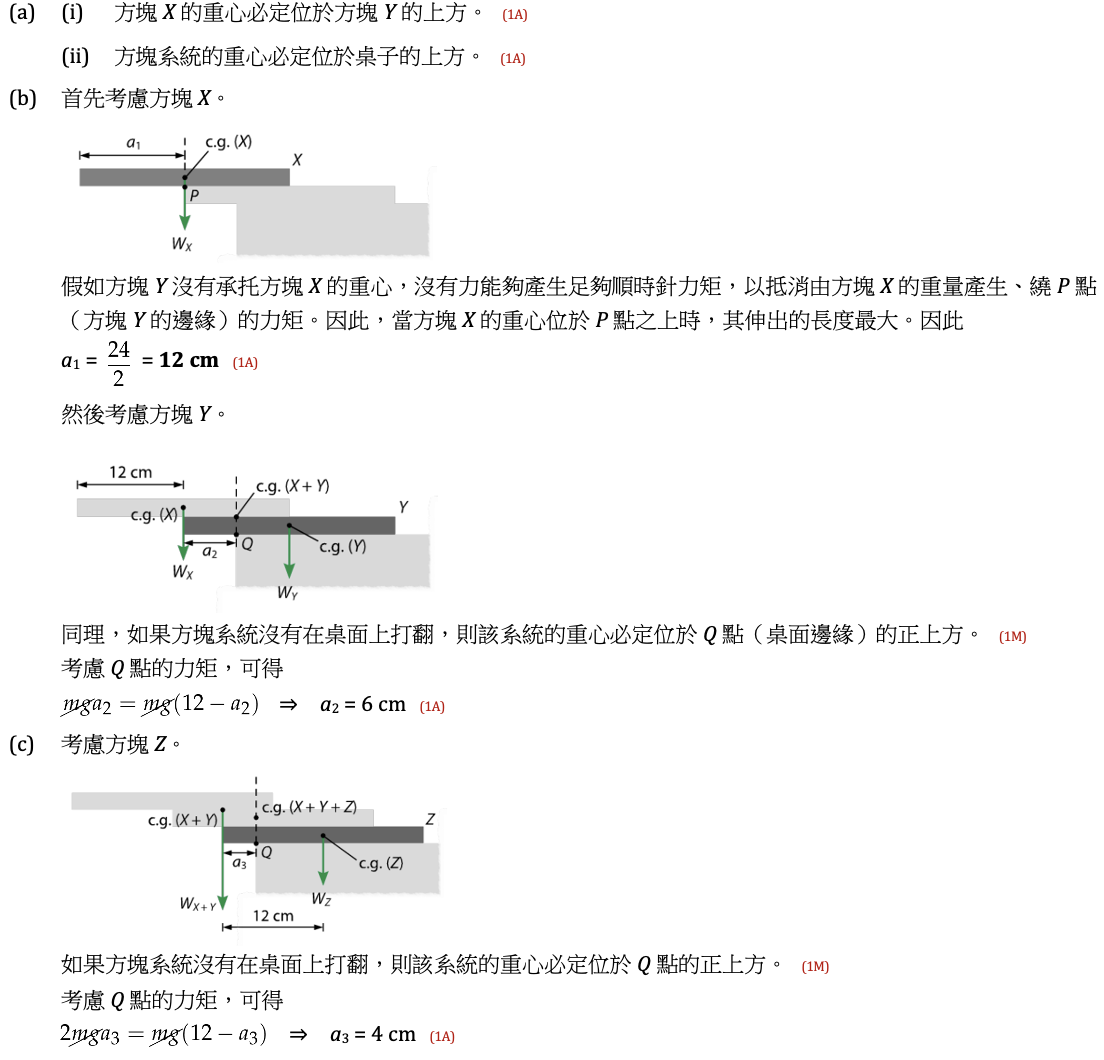
\includegraphics[width=\textwidth]{./img/ch3_moment_lq_2024-05-11-20-22-43.png}\par}
}